\begin{frame}{Reproduce article's figure}

\begin{columns} 
\begin{column}{0.5\textwidth}
    \begin{figure}
        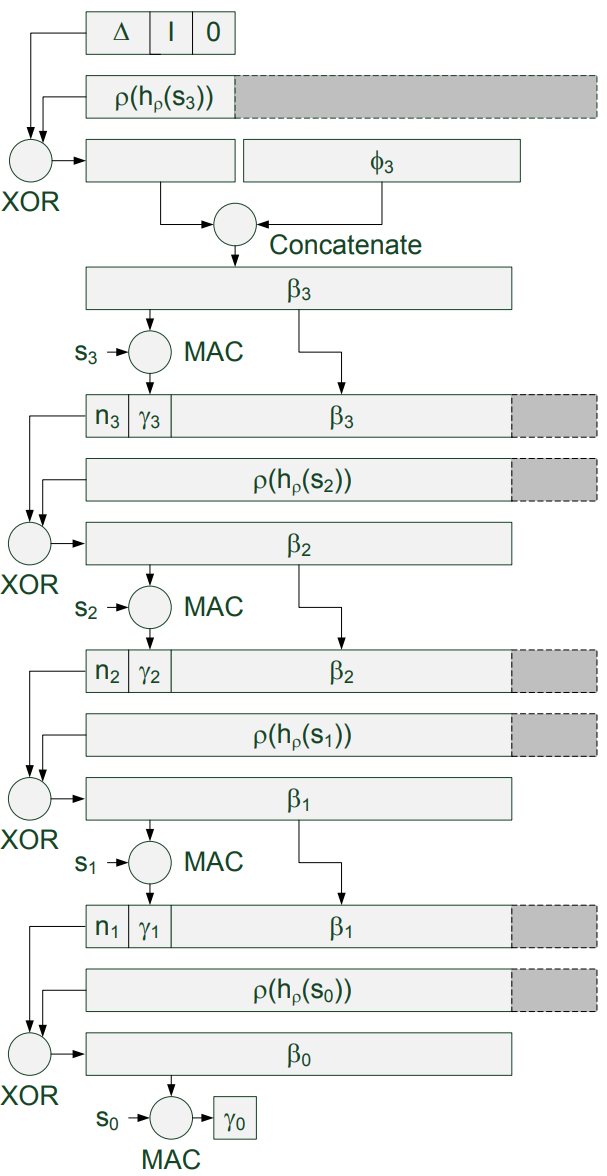
\includegraphics[scale=0.19]{Images/origin_beta_construction.png}
    \end{figure}
\end{column}

\vrule

\begin{column}{0.5\textwidth}\onslide<2->
\centering
\begin{tikzpicture}
    \setlength{\y}{0cm}

    \node (ip) [block=1] at (0, \y) {IP};
    \vgap
    \node (s3_) [block=7] at (0, \y) {};
    \node [inblock=1] at (0, \y) {$s_3$};
    \onslide<3-> {\node [inblock=1, three] at (0, \y) {$s_3$};}
    \node [inblock=6, gray] at (\width, \y) {}; 
    \vgap
    \node (s2_) [block=7] at (- 2*\width, \y) {};
    \node [inblock=3, gray] at (- 2*\width, \y) {}; 
    \node [inblock=4] at (3*\width - 2*\width, \y) {$s_2$};
    \onslide<3-> {\node [inblock=4, two] at (3*\width - 2*\width, \y) {$s_2$};}
    \vgap
    \node (s1_) [block=7] at (- 2*\width, \y) {};
    \node [inblock=3, gray] at (- 2*\width, \y) {}; 
    \node [inblock=2] at (3*\width - 2*\width, \y) {$s_1$};
    \onslide<3-> {\node [inblock=2, one] at (3*\width - 2*\width, \y) {$s_1$};}
    \node [inblock=2, gray] at (5*\width - 2*\width, \y) {};
    \vgap 
    \node (B3) [block=5] at (0, \y) {$\beta_3$}; 
    \onslide<3-> {
        \node [block_style=1, three] at (0, \y) {}; 
        \node [block_style=4, two] at (\width, \y) {}; 
        \node [block_style=2, one] at (\width, \y) {}; 
    }

    \node (xor3) [XOR] at (-3*\width, \y) {}; 
    \vGap
    \node (hmac3) [HMAC] at (1.5*\width, \y) {\tiny HMAC};
    \vGap
 
    \node (n3) [block=1] at (0, \y) {$n_3$}; 
    \node (y3) [block=1] at (\width, \y) {$\gamma_3$}; 
    \node (b3) [block=5] at (2*\width, \y) {$\beta_3$};
    \onslide<4-> {
        \node [block_style=1, three] at (2*\width, \y) {}; 
        \node [block_style=4, two] at (3*\width, \y) {}; 
        \node [block_style=2, one] at (3*\width, \y) {}; 
    } 
    \vgap
    \node (s2) [block=7] at (0, \y) {$s_2$};
    \onslide<5-> {\node [block_style=7, two] at (0, \y) {};}
    \vgap
    \node (B2) [block=5] at (0, \y) {$\beta_2$}; 
    \onslide<6-> {
        \node [block_style=1, three] at (2*\width, \y) {}; 
        \node [block_style=3, two] at (0*\width, \y) {}; 
        \node [block_style=2, one] at (3*\width, \y) {};
    } 
    \node (zero2) [zero_pad=2] at (5*\width, \y) {0}; 

    \node (xor2) [XOR] at (-\width, \y) {}; 
    \vGap
    \node (hmac2) [HMAC] at (1.5*\width, \y) {\tiny HMAC};
    \vGap

    \node (n2) [block=1] at (0, \y) {$n_2$}; 
    \node (y2) [block=1] at (\width, \y) {$\gamma_2$}; 
    \node (b2) [block=5] at (2*\width, \y) {$\beta_2$}; 
    \onslide<7-> {
        \node [block_style=1, three] at (4*\width, \y) {}; 
        \node [block_style=3, two] at (2*\width, \y) {}; 
        \node [block_style=2, one] at (5*\width, \y) {}; 
    } 
    \vgap
    \node (s1) [block=7] at (0, \y) {$s_1$};
    \onslide<8-> {\node [block_style=7, one] at (0, \y) {};}
    \vgap
    \node (B1) [block=5] at (0, \y) {$\beta_1$};
    \onslide<9-> {
        \node [block_style=1, three] at (4*\width, \y) {}; 
        \node [block_style=3, two] at (2*\width, \y) {}; 
        \node [block_style=5, one] at (0*\width, \y) {}; 
    } 
    \node (zero1) [zero_pad=2]  at (5*\width, \y) {0}; 

    \node (xor1) [XOR]  at (-\width, \y) {}; 
    \vGap
    \node (hmac1) [HMAC]  at (1.5*\width, \y) {\tiny HMAC};
    \vGap

    \node (n1) [block=1]  at (0, \y) {$n_1$}; 
    \node (y1) [block=1]  at (\width, \y) {$\gamma_1$}; 
    \onslide<1-9> {
        \node (b1) [block=5]  at (2*\width, \y) {$\beta_1$};
        % \node [block_style=1, three] at (6*\width, \y) {}; 
        % \node [block_style=3, two] at (4*\width, \y) {}; 
        % \node [block_style=5, one] at (2*\width, \y) {}; 
    }
    \onslide<10-> {
        \node (b1) [block=5]  at (2*\width, \y) {};
        \node [block_style=1, three] at (6*\width, \y) {}; 
        \node [block_style=3, two] at (4*\width, \y) {}; 
        \node [block_style=5, one] at (2*\width, \y) {}; 
        \node [block_style=1] at (2*\width, \y) {$n_2$}; 
        \node [block_style=1] at (3*\width, \y) {$\gamma_2$}; 
        \node [block_style=1] at (4*\width, \y) {$n_3$}; 
        \node [block_style=1] at (5*\width, \y) {$\gamma_3$}; 
        \node [block_style=1] at (6*\width, \y) {$IP$};
    }  

    %% XOR ARROWS %%
    % 3
    \draw[arrow] (ip.west) -- ++(-3*\width, 0) -- (xor3.north);
    \draw[arrow] (s3_.west) -- ++(-3*\width, 0) -- (xor3.north);
    \draw[arrow] (s2_.west) -- ++(-\width, 0) -- (xor3.north);
    \draw[arrow] (s1_.west) -- ++(-\width, 0) -- (xor3.north);
    \draw[arrow] (xor3.east) -- (B3.west);
    % 2
    \draw[arrow] (n3.west) -- ++(-\width, 0) -- (xor2.north);
    \draw[arrow] (s2.west) -- ++(-\width, 0) -- (xor2.north);
    \draw[arrow] (xor2.east) -- (B2.west);
    % 1
    \draw[arrow] (n2.west) -- ++(-\width, 0) -- (xor1.north);
    \draw[arrow] (s1.west) -- ++(-\width, 0) -- (xor1.north);
    \draw[arrow] (xor1.east) -- (B1.west);

    %% HMAC ARROWS %%
    % 3
    \node[left=\width of hmac3] (input_hmac3) {$s_3$};
    \onslide<4-> {\node[left=\width of hmac3] (input_hmac3) {\color{\sssColor}$s_3$};}
    \draw[arrow] (input_hmac3) -- (hmac3.west);
    \draw[arrow] (B3.south -| 1.5*\width, 0) -- (hmac3.north);
    \draw[arrow] (hmac3.south) -- (y3.north);
    % 2
    \node[left=\width of hmac2] (input_hmac2) {$s_2$};
    \onslide<7-> {\node[left=\width of hmac2] (input_hmac2) {\color{\ssColor}$s_2$};}
    \draw[arrow] (input_hmac2) -- (hmac2.west);
    \draw[arrow] (B2.south -| 1.5*\width, 0) -- (hmac2.north);
    \draw[arrow] (hmac2.south) -- (y2.north);
    % 1
    \node[left=\width of hmac1] (input_hmac1) {$s_1$};
    \onslide<10-> {\node[left=\width of hmac1] (input_hmac1) {\color{\sColor}$s_1$};}
    \draw[arrow] (input_hmac1) -- (hmac1.west);
    \draw[arrow] (B1.south -| 1.5*\width, 0) -- (hmac1.north);
    \draw[arrow] (hmac1.south) -- (y1.north);

    %% BETA ARROWS %%
    % 3
    \draw[arrowB] (B3.south) -- (b3.north);
    % 2
    \draw[arrowB] (B2.south) -- (b2.north);
    % 1
    \draw[arrowB] (B1.south) -- (b1.north);

\end{tikzpicture}
\end{column}

\end{columns}
\end{frame}